\documentclass[11pt,a4paper]{article}
\usepackage[utf8]{inputenc}
\usepackage[T1]{fontenc}
\usepackage[english]{babel}
\usepackage{lmodern}
\usepackage{microtype}
\usepackage{amsmath, amssymb, amsfonts}
\usepackage[margin=2.4cm]{geometry}
\usepackage{setspace}
\usepackage{url}
\usepackage{xurl}
\usepackage{booktabs}
\usepackage{tabularx}
\usepackage{graphicx}
\onehalfspacing

\title{\textbf{Stationary Strings Letter 2: No Source, No Agreement --- A Forensic Protocol for Literature Values\\
in Model-Assisted Physics}}
\author{Fahri Meral\\[0.2em]\small ORCID: 0009-0004-2287-2376}
\date{October 20, 2026}

\begin{document}

\maketitle

\begin{abstract}
We report a self-inflicted error in our own published-preprint series and
turn it into a transferable method. A table of experimental ratios for a
viscoelastic vortex experiment was labelled \emph{independent literature,
outside the model} and compared against two model outputs. The two model
outputs landed inside the two quoted intervals. The intervals were later
shown to exist in no source: four primary papers were downloaded and scanned
in full (PDF text \emph{and} LaTeX source), and the quoted numbers occur
nowhere in them. The claim was withdrawn. Two independent forensic tests are
introduced and released as code: \emph{repository archaeology}, which asks
whether a value ever carried a source record \emph{before} the agreement
that uses it was asserted, and \emph{source-existence scanning}, which asks
whether the quoted interval exists in the source corpus at all. We show that
the two apparent confirmations were algebraically dependent --- the second
ratio is the square of the first divided by a locked constant --- so the
apparent two-point agreement rested on a single degree of freedom resting
on a value with no source. Of the six literature quantities used in the two
affected tests, three could not be traced to any source and two more were
numerically wrong. We give a six-step detection protocol, state plainly what
the two tests can and cannot decide, and release the tool, its independent
self-test (7/7) and the forensic figure.
\end{abstract}

\section{The problem: intervals are the most dangerous artefact}
When a model output is compared with a literature value, the two natural
checks are \emph{is the number right?} and \emph{does the model agree?}.
Neither of them can detect a value that was never in the literature. A point
value that is wrong is caught the moment one opens the source; an
\emph{interval} that does not exist can only be caught by exhausting the
source, which is expensive and, unlike a wrong number, has no error
signature.

Three properties make intervals especially prone to this failure.
\begin{enumerate}
    \item \emph{They are cheap to invent and hard to falsify.} Two round
    numbers read as a measurement. ``$r \in [1.55,1.70]$'' looks exactly
    like a summary of a figure axis.
    \item \emph{They are self-sealing.} If a model value happens to land
    inside the interval, the agreement appears to confirm the value --- and
    the value appears to confirm the model. No external check is triggered.
    \item \emph{They evade the falsification asymmetry.} A wrong point value
    propagates a wrong prediction. A phantom interval propagates a wrong
    \emph{confirmation}, which is worse, because it is not visible in any
    downstream computation.
\end{enumerate}
This letter is a case study of exactly that failure, in our own work, with
the forensic method and the released tool.

\section{The case}
In the preprint series later numbered SS-XIV, test T35 compared the
dimensionless ratios predicted for a 100\,ppm polyacrylamide-oxide solution in
a two-disk tank against two quoted intervals,
\begin{equation}
\label{eq:bands}
r_{\mathrm{PEO}}/r_{\mathrm{water}} \in [1.55,\,1.70],
\qquad
\Delta h_{\mathrm{PEO}}/\Delta h_{\mathrm{water}} \in [0.30,\,0.35],
\end{equation}
labelled \emph{independent literature (model-external)}. The model outputs
were
\begin{equation}
\label{eq:model}
r_{\mathrm{PEO}}/r_{\mathrm{water}} = 1.626037936551738,
\qquad
\Delta h_{\mathrm{PEO}}/\Delta h_{\mathrm{water}} = 0.314025361279003,
\end{equation}
and Eq.~\eqref{eq:model} lies inside Eq.~\eqref{eq:bands} in both cases ---
the intervals were read off as confirmations.

\subsection{Provenance of the intervals}
\begin{itemize}
    \item The quoted intervals entered the repository in commit
    \texttt{043f2ee} (19 October 2026, 20:14), already in the
    \emph{independent literature} frame, in the same commit that asserted
    the agreement.
    \item A source audit 56 minutes later (commit \texttt{96467dd},
    21:10) downloaded four primary papers and scanned them in full:
    Groisman \& Steinberg (2000) \cite{gs2000}; van Buel \& Stark (2022)
    \cite{vbs2022}; Guido et al.\ (2021) \cite{guido2021}; Burghelea et al.\
    (2006) \cite{bss2006}.
    \item In the LaTeX source of Groisman \& Steinberg the strings
    \texttt{1.55}, \texttt{1.70}, \texttt{0.30}, \texttt{0.35},
    \emph{funnel}, \emph{dimple}, \emph{core} and \emph{free surface} do not
    occur at all; the extracted PDF text (19\,519 characters) contains
    neither \texttt{1.55} nor \texttt{1.70}. That experiment is
    polyacrylamide plus syrup between two parallel disks, $d/R = 0.263$, and
    its figure inventory (schematic; $\sigma/\sigma_{\rm lam}$ versus
    $\dot\gamma$; snapshots; two Fourier spectra) contains no free-surface or
    dimple measurement of any kind.
    \item The intervals were therefore withdrawn and the comparison removed.
\end{itemize}
The underlying physics is real and sourceable --- the same literature
reports a flow-resistance increase factor $\sigma/\sigma_{\rm lam} = 12$ and
$19$ for 10 and 20\,mm gaps, a critical Weissenberg number
$\mathrm{Wi}_c = 12$, and a boundary-layer thickness as the new length
scale of elastic turbulence --- but the quoted interval pair is traceable to
nothing.

\section{The two forensic tests}
\subsection{Repository archaeology}
The first test does not look for the value in the literature at all; it looks
for it in the project's own history. A literature value that was transcribed
from a source must, at some point, have been written down \emph{as a
literature value} before the model output was compared with it. We
therefore compare three first appearances in the commit history:
\begin{align}
t_{\mathrm{first}} &:\ \text{first standalone occurrence of the token},\\
t_{\mathrm{ref}} &:\ \text{first occurrence in a reference frame},\\
t_{\mathrm{claim}} &:\ \text{first occurrence in an agreement claim}.
\end{align}
If $t_{\mathrm{ref}} = t_{\mathrm{claim}}$, the value was born as an
agreement: there is no earlier record in which it was a sourced datum, and
the label \emph{independent literature} was applied at the moment of the
claim rather than derived from a source.

Two implementation details matter and are enforced in the released tool.
First, the search must be for the \emph{standalone token}: a substring
search for \texttt{1.55} finds the unrelated quantity \texttt{1.556152e+05}
in the project's first commit and would manufacture a false provenance
record. Second, the reference and claim frames are detected in a window of
$\pm3$ lines, because a citation and its number are routinely split across
two lines.

\subsection{Source-existence scanning}
The second test asks whether the quoted interval exists in the source corpus
at all: every arXiv LaTeX source and every PDF in the corpus is searched for
the number with token boundaries, and the number of files in which the
members of an interval co-occur is reported separately. The scan must
report failures explicitly; a PDF whose text cannot be extracted is counted
as an error, never as a zero.

The results for the corpus of 100 files (81 PDFs, of which 17 are the
primary papers, and 19 arXiv LaTeX source files) are:
\begin{table}[!htbp]
\centering\footnotesize
\setlength{\tabcolsep}{5pt}
\caption{\textbf{Existence scan of the literature values used in T35 and T36.}
Corpus: 100 files (81 PDFs + 19 arXiv LaTeX sources). Matches are counted with
token boundaries. \emph{Co-occurrence} counts the files in which all members
of an interval appear together.}
\label{tab:scan}
\vspace{0.1cm}
\begin{tabular}{@{}llrr@{}}
\toprule
Value & Repository verdict & Matches & Co-occurrence \\
\midrule
\texttt{1.55} & GHOST\_CANDIDATE & 0 & --- \\
\texttt{1.70} & GHOST\_CANDIDATE & 0 & --- \\
\texttt{1.55\,+\,1.70} (interval) & GHOST\_CANDIDATE & 0 & 0 \\
\texttt{0.30} & GHOST\_CANDIDATE & 4 & --- \\
\texttt{0.35} & HAS\_PROVENANCE & 5 & --- \\
\texttt{0.30\,+\,0.35} (interval) & GHOST\_CANDIDATE & 9 & 3 \\
\texttt{2.25} (glitch band) & GHOST\_CANDIDATE & 2 & --- \\
\texttt{0.0160} ($I_{\rm crust}/I$) & GHOST\_CANDIDATE & 0 & --- \\
\texttt{0.014} ($I_{\rm crust}/I$, corrected) & GHOST\_CANDIDATE & 4 & --- \\
\bottomrule
\end{tabular}
\end{table}

Table~\ref{tab:scan} contains the lesson of the whole letter in two lines.
The numbers \texttt{1.55} and \texttt{1.70} occur nowhere, so the interval
is phantom. But \texttt{0.30} and \texttt{0.35} \emph{do} occur, four and
five times, and they co-occur in three files --- a 511\,keV line-modelling
paper, an antihydrogen hyperfine paper and two INTEGRAL flux maps --- in
contexts with nothing to do with viscoelastic vortices. \emph{Token presence
is not provenance, and co-occurrence without context is not provenance
either.} Only the semantic reading of the source settles it, which is
precisely why the cheapest automatable test --- the archaeology --- has to be
run first, while the claim is still cheap to withdraw.

\subsection{The two apparent confirmations were one}
The two agreements in Eq.~\eqref{eq:bands} are algebraically dependent. With
$a \equiv \mathcal{C}_{\mathrm{univ}}$ and the locked $\mu_s$,
\begin{equation}
\label{eq:dep}
\frac{\Delta h_{\mathrm{PEO}}}{\Delta h_{\mathrm{water}}}
= \frac{1}{a^{2}(1+\mu_s)}
= \left(\frac{u_{\max}^{\mathrm{PEO}}}{u_{\max}^{\mathrm{water}}}\right)^{2}
\frac{1}{1+\mu_s},
\end{equation}
because the free-surface depression scales as the inverse square of the
Burgers core radius, $r_c \propto a$. Numerically the identity in
Eq.~\eqref{eq:dep} holds to $5.6\times10^{-17}$, and
$r_{\mathrm{PEO}}/r_{\mathrm{water}} = \mathcal{C}_{\mathrm{univ}}$ to
$2.2\times10^{-16}$. The second interval agreement is therefore a
reparametrisation of the first, not an independent test of it: the pair
rests on a single degree of freedom. Combined with the fact that the
intervals were phantom, the apparent two-point confirmation collapses to
zero.

\section{The protocol}
Six steps, of which only the first three are new practice for most authors.
\begin{enumerate}
    \item \textbf{Quote a source line for every literature value.} A file,
    a table or figure number, and a page. ``Literature'' without a
    locatable location is not a citation.
    \item \textbf{Ask whether the source \emph{contains} it.} The question
    is existence, not equality. For an interval, ask whether both members
    appear together, in the same context.
    \item \textbf{Scan the machine-readable source.} For arXiv papers, the
    LaTeX source finds figure captions, table notes and supplementary
    material that a PDF text extraction misses, and it makes the search
    reproducible.
    \item \textbf{Recover the first appearance.} A version-controlled
    project keeps a time-stamped record of when each value entered and in
    which frame. The search must respect token boundaries.
    \item \textbf{Test the ordering.} A value called independent must have
    been recorded as sourced \emph{before} the agreement that uses it. If
    the first reference and the first claim are the same commit, the
    independence was asserted, not derived.
    \item \textbf{Withdraw rather than repair.} When the number cannot be
    traced, the claim citing it is withdrawn even if the physics survives.
    Replace it with the value that \emph{is} sourceable, and record the
    withdrawal.
\end{enumerate}
Step 6 is the expensive one and the reason step 1 is cheap: a withdrawal
costs a paragraph, whereas an untraceable confirmation costs the reader the
ability to trust the rest of the table.

\section{What the two tests can and cannot decide}
We state the limits explicitly, because a forensic tool that overstates its
reach becomes the next ghost.
\begin{itemize}
    \item \emph{The archaeology test says nothing about truth.} It reports
    whether a value carried a source record in \emph{this} repository
    before it was used in a claim. The corrected crust-fraction value
    $\Delta I/I \ge 0.014$ is genuinely sourced (it occurs in the LaTeX
    source of Link et al.~\cite{link1999}) and is nevertheless flagged,
    because the repository had never transcribed that source before the
    audit. A flag is a request for a source line, not a refutation.
    \item \emph{The repository cannot establish origin.} It establishes only
    that no provenance record exists. Whether the interval was misremembered,
    carried over from an earlier working note, suggested by a language model
    during drafting, or produced by a slip cannot be determined from the
    repository, and we do not claim it.
    \item \emph{The existence scan bounds the printed record, not the
    physics.} Zero matches means the quoted numbers appear nowhere in the
    scanned corpus; it does not prove that no measurement resembling them was
    ever made. What it does prove is that the claim as written had no
    retrievable basis.
\end{itemize}

\section{The scale of the problem in one test pair}
The audit of tests T35 and T36 used six literature quantities: the two
intervals, the glitch amplitude $(2.25\pm0.35)\times10^{-6}$, the healing
fraction $Q\in[0.05,0.18]$, the crust-fraction ratio $I_{\rm crust}/I$, and
the glitch relaxation timescales. Three could not be traced to any source;
two more were numerically wrong and were replaced by measured values
($I_{\rm crust}/I = 0.0160 \rightarrow \ge 0.014$ from Link et al., and
arbitrary 6- and 60-day relaxation times $\rightarrow$ measured 1.2\,min,
0.53, 3.29 and 19.07\,days from Dodson et al.~\cite{dodson2002}); only the
sixth was already correct. \textbf{Five of six required correction.} In this
series that ratio improved to zero only because the sources were eventually
downloaded and read.

\section{Reproducibility}
The complete forensic machinery is released with this letter:
\begin{itemize}
    \item \texttt{ghost\_audit.py} --- the two tests: repository archaeology
    (first appearance, reference frame, claim frame, with token-boundary
    enforcement and a $\pm3$-line context window) and source-existence
    scanning (with explicit co-occurrence counting and explicit failure
    reporting).
    \item \texttt{mini\_check\_l2.py} --- an independent self-test that
    builds synthetic repositories and corpora and checks the four verdicts
    (\texttt{GHOST\_CANDIDATE}, \texttt{HAS\_PROVENANCE},
    \texttt{NOT\_A\_LIT\_VALUE}, \texttt{ABSENT}), the token-boundary rule,
    the co-occurrence count and the real case: 7/7 pass.
    \item Figure 1 --- the life cycle of the phantom interval, the existence
    scan, the algebraic collapse of the two apparent confirmations, and the
    protocol.
\end{itemize}
The tool does not import the solver and does not depend on the physical
model; it operates on a repository and a corpus. Execution instructions are
given in the accompanying repository.

\clearpage
\begin{figure}[!htbp]
\centering
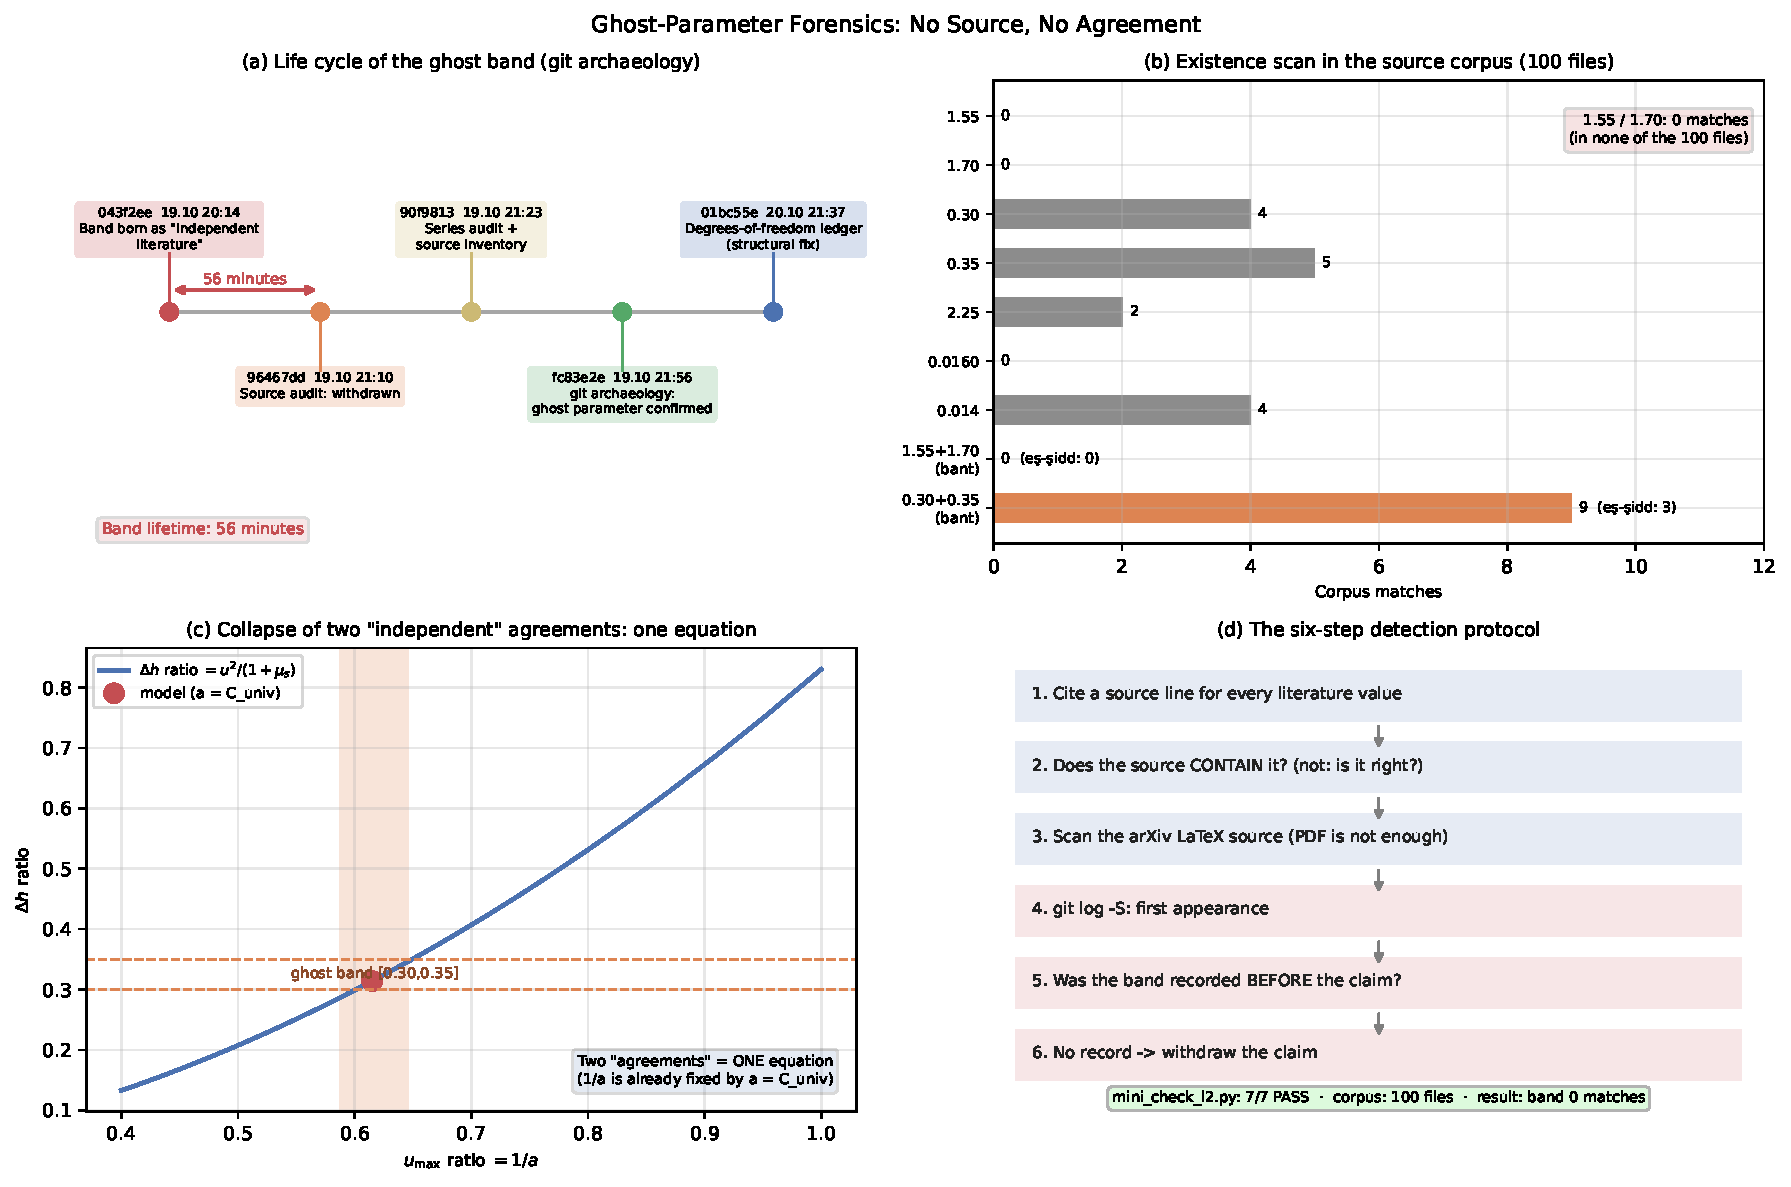
\includegraphics[width=\textwidth]{../figs/fig16_ghost_parameter_forensics_en.pdf}
\caption{\textbf{Forensic summary of the phantom interval.}
(a) The interval was created as \emph{independent literature} in commit
\texttt{043f2ee} and withdrawn 56 minutes later by the source audit; the
archaeology confirmation and the structural fix (the degrees-of-freedom
ledger) follow. (b) Existence scan of the source corpus: \texttt{1.55} and
\texttt{1.70} occur nowhere; \texttt{0.30} and \texttt{0.35} occur, and
co-occur in three files, but in unrelated contexts. (c) The two apparent
confirmations are one equation: the depression ratio is the square of the
velocity ratio divided by $1+\mu_s$. (d) The six-step protocol.}
\label{fig:ghost}
\end{figure}

\clearpage
\begin{thebibliography}{99}
    \bibitem{gs2000} Groisman, A. A. \& Steinberg, V. (2000). Elastic
    turbulence in a polymer solution. \textit{Nature \textbf{405}}, 53--61.
    arXiv:nlin/0104052.
    \bibitem{vbs2022} van Buel, J. \& Stark, P. D. (2022). Elastic turbulence
    in dilute polymer solutions. arXiv:2202.12714.
    \bibitem{guido2021} Guido, S. \textit{et al.} (2021). Development of
    vortex based on polymeric solution. arXiv:2110.03004.
    \bibitem{bss2006} Burghelea, A., Segre, D. \& Steinberg, V. (2006).
    Elastic turbulence in a dilute polymer solution.
    arXiv:physics/0609112.
    \bibitem{link1999} Link, F., Epstein, D. L. \& Lattimer, J. M. (1999).
    Glitching pulsars. \textit{Phys.\ Rev.\ Lett.\ \textbf{83}}, 3807--3810.
    \bibitem{dodson2002} Dodson, R. N. \textit{et al.} (2002). Frequency
    behaviour of the Vela pulsar during the glitch of 2000 January.
    \textit{Astrophys.\ J.\ \textbf{574}}, 471--475.
    arXiv:astro-ph/0201005.
\end{thebibliography}

\end{document}
